% Source: graduate-coursework/Sp26/CSCE775/course_notes/mc_prediction_guide.tex
% Description: The $3\times 3$ gridworld. $S_9$ (garnet) is the terminal goal state.

\documentclass[border=4pt]{standalone}
\usepackage{amsfonts}
\usepackage{amsmath}
\usepackage{amssymb}
\usepackage{amsthm}
\usepackage[T1]{fontenc}
\usepackage{graphicx}
\usepackage{tikz}
\usepackage{xcolor}
\usetikzlibrary{arrows.meta, positioning, shapes.geometric, calc, decorations.pathreplacing}

\definecolor{Garnet}{HTML}{73000a}
\definecolor{SecondaryBlue}{HTML}{466A9F}
\definecolor{SecondaryGreen}{HTML}{65780B}
\definecolor{FlatRed}{HTML}{CC2E40}
\definecolor{FlatDark}{HTML}{1F414D}
\definecolor{FlatYellow}{HTML}{CED318}
\definecolor{FlatGold}{HTML}{A49137}
\definecolor{LightGray}{HTML}{F0F0F0}
\definecolor{Rose}{HTML}{CC2E40}

\renewcommand{\baselinestretch}{1.2}
\newcommand{\vocab}[1]{\textbf{\textcolor{Garnet}{#1}}}
\newcommand{\mathhighlight}[1]{\textcolor{SecondaryBlue}{#1}}

\begin{document}
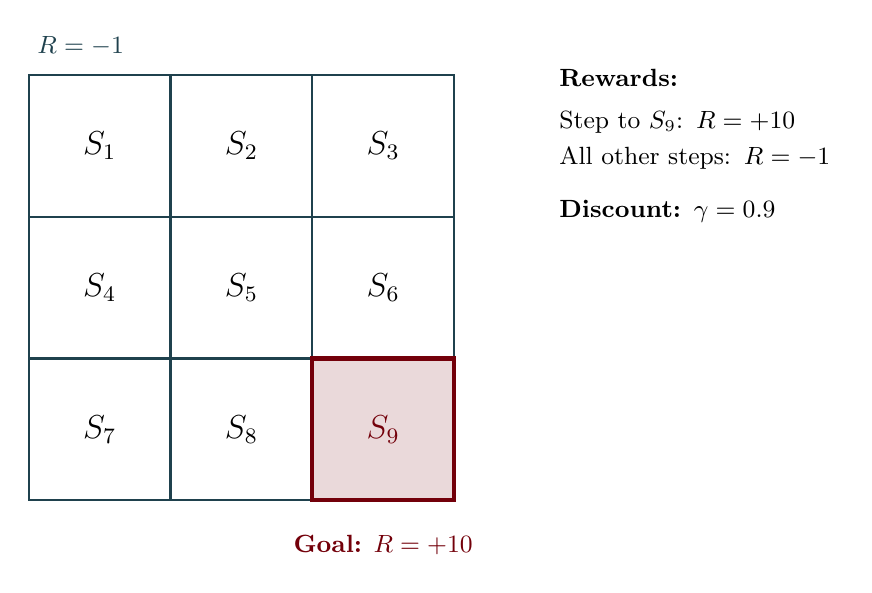
\begin{tikzpicture}[
    cell/.style={minimum size=1.8cm, draw=FlatDark, thick, font=\large},
    goal/.style={cell, fill=Garnet!15, draw=Garnet, line width=1.5pt},
    rlabel/.style={font=\small, FlatDark}
]
% Row 1 (top): S1, S2, S3
\node[cell] (s1) at (0, 3.6) {$S_1$};
\node[cell] (s2) at (1.8, 3.6) {$S_2$};
\node[cell] (s3) at (3.6, 3.6) {$S_3$};
% Row 2: S4, S5, S6
\node[cell] (s4) at (0, 1.8) {$S_4$};
\node[cell] (s5) at (1.8, 1.8) {$S_5$};
\node[cell] (s6) at (3.6, 1.8) {$S_6$};
% Row 3 (bottom): S7, S8, S9
\node[cell] (s7) at (0, 0) {$S_7$};
\node[cell] (s8) at (1.8, 0) {$S_8$};
\node[goal] (s9) at (3.6, 0) {\textcolor{Garnet}{$S_9$}};

% Reward labels
\node[rlabel, above=0.1cm of s1.north west, anchor=south west] {$R = -1$};
\node[rlabel, below=0.3cm of s9] {\textcolor{Garnet}{\textbf{Goal:} $R = +10$}};

% Legend
\node[right=1.2cm of s3, anchor=west, font=\small, text width=3.5cm] {
    \textbf{Rewards:}\\[2pt]
    Step to $S_9$: $R = +10$\\
    All other steps: $R = -1$\\[6pt]
    \textbf{Discount:} $\gamma = 0.9$
};
\end{tikzpicture}
\end{document}
